\documentclass[a4paper,twoside]{article}
\usepackage{amsmath}
\usepackage{amsfonts}
%\usepackage{mathabx} %for the \wdcheck
\usepackage{amssymb}
\usepackage{caption}
\usepackage[english]{babel}
\usepackage{bibgerm}
\usepackage[utf8]{inputenc}
\usepackage[T1]{fontenc}
\usepackage{graphicx}
\usepackage{latexsym}
\usepackage{subcaption} 
\usepackage[inner=36pt, textwidth=345pt]{geometry}
\usepackage{subfiles}
\usepackage{siunitx}
\usepackage{tikz}
\usepackage{tikz-feynman}
\usetikzlibrary{shapes.geometric}
\usetikzlibrary{decorations.pathmorphing}
\usepackage{twemojis}
\usepackage{hyperref}
\usepackage[makeroom]{cancel}
\usepackage{pdfpages}
\usepackage{bm}
\usepackage{ relsize }
\usepackage{float}
\usepackage{cancel}
\usepackage{stmaryrd}
\usepackage{TamwynLatexLib}

\usepackage{bbm} %for the \mathbb{1}
\newcommand{\indc}{\mathlarger{\mathlarger{\mathbbm{1}\normalsize}}}


%\input{C:/Users/Tamwyn/Documents/CustomLatexTextMF/mytexmf/tex/latex/UniLaTeXPackage/Arto/ArtoMain.tex}


\geometry{a4paper, top=15mm, left=28mm, right=28mm, bottom=20mm,
headsep=10mm, footskip=12mm}
%\thispagestyle{empty}
\setlength\parindent{0pt}

\begin{document}
\thispagestyle{empty}
\begin{center} 
    \vspace*{40pt}
    \noindent\Huge.\\
    \noindent$\circ$\\
    \rule{0.1\textwidth}{0.75pt}\\
    \rule[20pt]{0.17\textwidth}{0.75pt} \rule[20pt]{0.5\textwidth}{0.75pt} \rule[20pt]{0.17\textwidth}{0.75pt}\\
    \vspace*{30pt}
    \Huge $\mathcal{P}$\textit{roximity} $\mathcal{E}$\textit{ffects}\\
     \textit{in}\\ 
    $\mathcal{A}$\textit{ltermagnetic}  $\mathcal{S}$\textit{ystems}
    \vspace*{12pt}\\
    $~\sim\circ\sim~$
    \vspace*{48pt}\\
    \normalsize
 a bachelor thesis.\\

\end{center}
\vspace*{60pt}
\noindent
\normalsize
\textbf{Written by} Arto Steffan, \\
\textbf{under the supervision of} prof. dr. Jacob Wüsthoff Linder, \\
\textbf{and corrected by} prof. dr. Wolfgang Belzig.\\
\vspace*{124pt}
\begin{center}
    \rule{.4\textwidth}{0.4pt}
\end{center}
\vspace*{12pt}
\begin{figure}[H]
    \centering
    \begin{subfigure}{0.45\textwidth}
        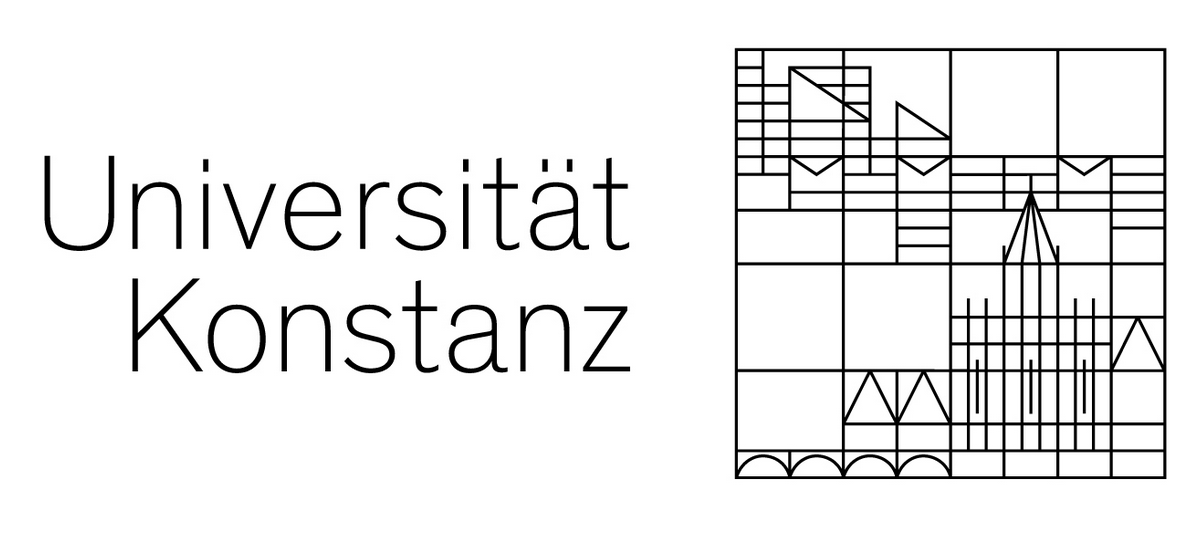
\includegraphics[width=.8\textwidth]{Ressources/UniKn.png}
    \end{subfigure}\hspace*{0.1\textwidth}
    \begin{subfigure}{0.45\textwidth}
        
\includegraphics[width=0.9\textwidth]{Ressources/ntnu.png}
        \vspace*{12pt}
    \end{subfigure}
\end{figure}
\newpage

\subfile{Pages/0_Acknolegmend.tex} 
\vspace*{7pt}
\newpage

% -----------------------------------------------------------
% Inhaltsvorbereitung

    \tableofcontents
    \thispagestyle{empty}	
    \setcounter{page}{1}
    \pagenumbering{arabic}



% -----------------------------------------------------------

\subfile{Pages/1_Introduction.tex} 
\subfile{Pages/2_TheoreticalBackground.tex} 
\subfile{Pages/3_BdGFormalism.tex} 


%-----------------------------------------------------------
% Abspann und Credits

%\newpage
%    \subfile{Sections/5-Literatur.tex}
%\newpage
%    \listoffigures
%    \listoftables


%\includepdf[pages=1-1,scale=0.9,frame=true]{Protokolle/PATH.pdf}
\end{document}